\documentclass[10pt,a4paper]{article}
\usepackage[utf8]{inputenc}
\usepackage[italian]{babel}
\usepackage{amsmath}
\usepackage{xcolor}
\usepackage{siunitx}
\usepackage{circuitikz}
\usepackage{amsfonts}
\usepackage{amssymb}
\usepackage{graphicx}
\usepackage{siunitx}
\usepackage[left=2cm,right=2cm,top=2cm,bottom=2cm]{geometry}
\newcommand{\rem}[1]{[\emph{#1}]}
\newcommand{\exn}{\phantom{xxx}}
\renewcommand{\thesubsection}{\thesection.\alph{subsection}}  %% use 1.a numbering

\author{Gruppo 1G.BN \\ Massimo Bilancioni, Alessandro Foligno, Giuseppe Zanichelli }
\title{Es06B:Usi non lineari dell’ OpAmp }
\begin{document}
	\date{8 novembre 2018}
	\maketitle
	
	
	\section*{Scopo dell' esperienza}
	Scopo dell'esperienza è l'analisi di circuiti che fanno usi non lineari dell'Amplificatore Operazionale




\section{Ampificatori di Carica}
	\subsection{Montaggio circuito e valore delle componenti}
		Si monta il circuito sulla basetta.
		I valori delle varie componenti sono i seguenti:
		\\$C_T=0.967\pm 0.04$ \si{\nano\farad}\\$C_f=0.958\pm 0.04$ \si{\nano\farad}\\$R_2=99.9\pm 0.9 $ \si{\ohm}\\$R_1=0.392 \pm0.03   $ \si{\mega \ohm}\\
				Il potenziometro, invece, ha una resistenza massima di circa 1\si{\mega\ohm}
	\subsection{Analisi dei segnali}
		Studiando il circuito, ci si aspetta, in $V_{disc}$ un'onda quadra di duty cycle variabile e ampiezza data dalle tensioni di alimentazioni dell'op-amp, dove il segnale alto indica quando il segnale in $V_{sh}$ è sopra la soglia.
		Per quanto riguarda la prima parte del circuito, anzitutto osserviamo che, ad ogni cambio di polarità dell'onda quadra, viene iniettata nel circuito una quantità di carica pari a $Q=V_{pp} C_T$. Questo "impulso" di corrente deve tutto sul condensatore $C_F$ dato che sulla resistenza non c'è abbastanza ddP per farlo passare.
		Dopo che il condensatore riceve la carica inizia a scaricarsi. Ci si aspetta, quindi, come ampiezza massima del segnale $V_{sh}$, $V_{max}=\frac{Q}{C_F}=2 V_{in} \frac{C_T}{C_F}\approx 2 V_{in} $ dato che le capacità sono più o meno uguali. Infatti, con un'onda quadra in ingresso $V_in\approx3V$ si osserva il segnale $V_{sh}$ riportato in Figura \ref{fig:sample}, di ampiezza $\approx 6V$.
		\begin{figure}
			\centering
			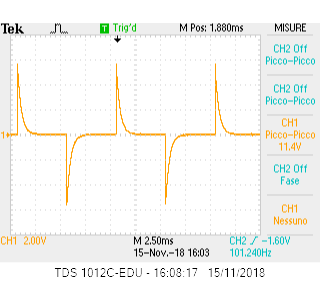
\includegraphics{sample.png}
			\caption{segnale $V_{sh}$}
			\label{fig:sample}
		\end{figure}
	
\clearpage	
\section{ MULTIVIBRATORI }


\subsection{Multivibratore astabile}
I valori misurati di $R_1$, $R_2$ e $R_3$ sono:
\[ R_1 = (9.75\pm 0.08)\si{\kilo\ohm} \qquad  R_2 = (9.98 \pm 0.08)\si{\kilo\ohm} \qquad   R_3 = ( 0.994 \pm0.001 ) \si{\kilo\ohm}\]

a)  Il periodo di oscillazione del circuito in figura è : \[ T = 2 RC \log( 1+ 2 R_2/R_1)\]





b) Abbiamo scelto i seguenti valori per la resistenza e la capacità:
\[ R = ( 46.0 \pm0.5 )\si{\kilo\ohm} \qquad   C = (21.3\pm0.9 )\si{\nano \farad}\]

a cui corrisponde un periodo di oscillazione teorico:
\[T_{att}= (2.18\pm 0.14 )\si{\milli \second}\]



c) \rem{ foto oscilloscopio Vout v+ e v- , misurare periodo oscill,  vout = ddp clamp morse,v+ e v- insieme per vedere confronto ampiezze}
Le misure picco picco per  segnali  $V_{out}, v_{+}$ e $v_{-}$ sono :
\[ V_{out,pp}= (13.6\pm 0.2)\si{\kilo\ohm} \qquad  v_{+,pp}= (6.88 \pm 0.12)\si{\kilo\ohm} \qquad   v_{-,pp}= ( 7.04 \pm0.08 ) \si{\kilo\ohm}\]
Il periodo misurato dell'oscillazione misurato sull'oscilloscopio da come risultato :
\[ T = (2.26 \pm 0.02)\]




\begin{figure}[h]
	\begin{center}
		
			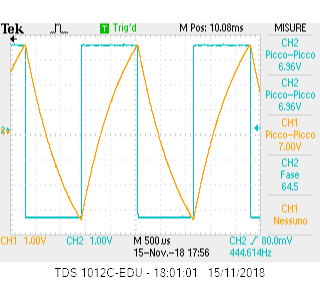
\includegraphics[scale=0.8]{v+_v-.png}
		\caption{\small i segnali $V_+$( in azzurro ) e $ V_-$ ( in arancione )  multivibratore astabile}

		\label{fig:v+v-}
	\end{center}

\end{figure}



\begin{figure}[h]
	\begin{center}
		
			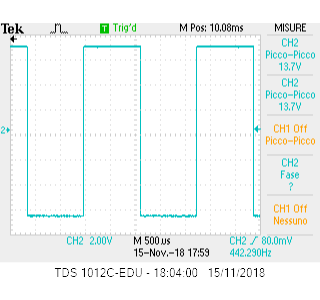
\includegraphics[scale=0.8]{vout_punto2.png}
		\caption{\small segnale $V_{out}$ del multivibratore astabile }

		\label{fig:v+v-}
	\end{center}

\end{figure}


d) La serie dei due  diodi  Zener limita l'escursione in tensione, infatti deve essere $|V_{out}| \le V_{\gamma} +V_{z} = V_{Max}$.
 Se $V_{1}$ (segnale all'uscita dell'Op-Amp) fosse maggiore dii $V_{max}$ si avrebbe un cortocircuito; per evitare questa eventualità si introduce  una resistenza $R_3$ che limita la corrente.

Dalla misura risulta \[V_{max} = ( 6.8\pm 0.1) \si \volt\]






\end{document}          
